\section{Stack Procedures}

\label{sec:4.Stack}

The following sub-section only discusses the design architecture of the Stack "\textit{class}", detailed explanations of the procedures will be covered further in the subsequent sub-sections.

\subsection{Stack Design Architecture}
    The Stack "\textit{class}" is designed by dividing a memory area \texttt{.space} into 3 parts. The first part holds the address of the word after the top of the stack, the next word is an integer indicating the number of elements inserted into the stack, and the remaining part is divided into word-sized regions containing the values of the elements pushed onto the stack [\ref{fig:4.StackArchitecture}]. If a Push operation exceeds the memory area, the system will report a stack overflow error, and if a \texttt{TOP} or \texttt{POP} operation is performed when the stack is empty, the system will report a stack underflow error.
    
    \begin{figure}[htbp]
        \centering
        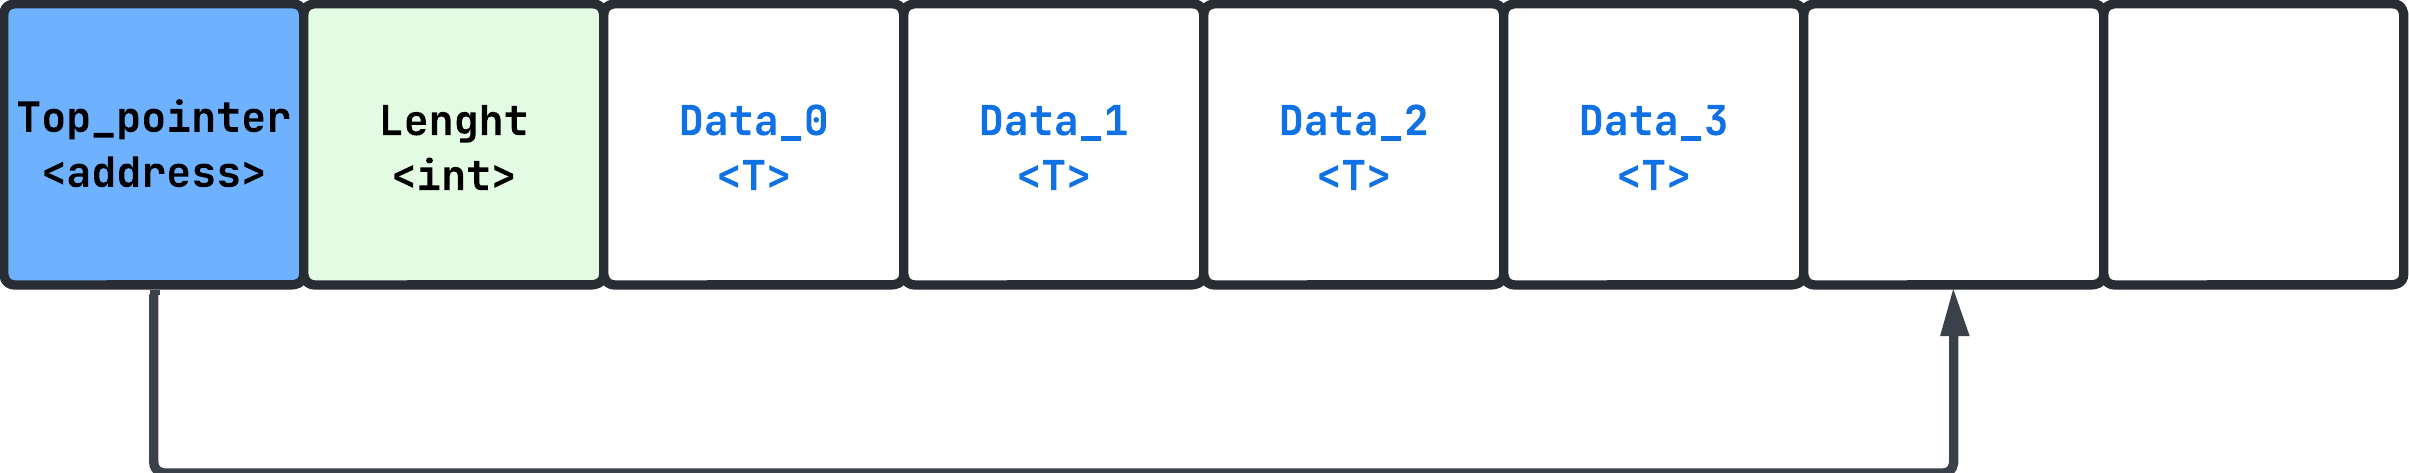
\includegraphics[width=1\textwidth]{graphics/3.StackArchitecture.png}
        \caption{Stack implementation architecture}
        \label{fig:4.StackArchitecture}
    \end{figure}
    
    An example of how data is organized in a stack:

    Let's push the each char \(HCMUT\) onto the stack sequentially. The result [\ref{fig:4.StackPrintMar}] shows that the first word at address \texttt{0x10010020} points to the address \texttt{0x1001003c}, meaning the word after the \texttt{TOP}.

    \begin{code}{ASM}
        la $a0, stack   # Load address of .space
        
        # STACK_PUSH($a0 = address of memory block, $a1 = value) => void
        li $a1, H
        jal STACK_PUSH
        li $a1, C
        jal STACK_PUSH
        li $a1, M
        jal STACK_PUSH
        li $a1, U
        jal STACK_PUSH
        li $a1, T
        jal STACK_PUSH
        
        la $a1, PRINT_CHAR
        jal PRINT_STACK
    \end{code}

\begin{figure}[htbp]
    \centering
    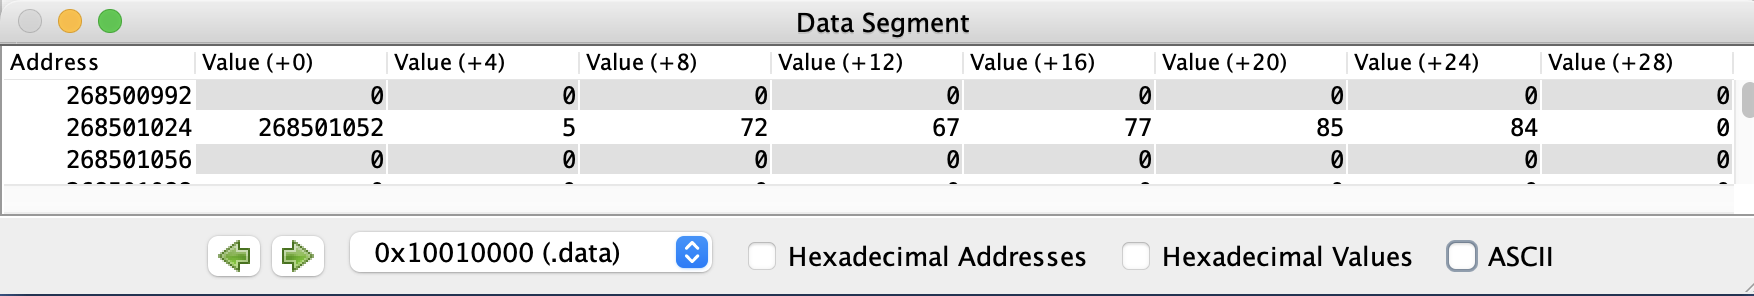
\includegraphics[width=1\textwidth]{graphics/3.StackPrintMar.png}
    \caption{Stack memory architecture}
    \label{fig:4.StackPrintMar}
\end{figure}

\subsection{Stack Procedures API}
    This sub-section contains all the MIPS32 procedures API for the Stack "\textit{class}". All procedures below use register \texttt{\$a0} to pass the address of the memory block containing the address of the \texttt{Top\_pointer} (the blue block in figure [\ref{fig:4.StackArchitecture}]). All procedures have time complexity of \(O(1)\), except \texttt{STACK\_RESET} and \texttt{STACK\_PRINT} have complexity of \(O(n)\).

    \begin{longtable}{|m{3cm}|m{3cm}|m{2cm}|m{1cm}|m{5.1cm}|}
        \hline
            \textbf{Procedure} & 
            \textbf{Args} \newline (\texttt{\$a0} = \textit{memory block address}) & 
            \textbf{Return} & 
            \centering \textbf{Leaf fucnt} &
            \textbf{Description}\\
        \hline
        \endfirsthead
        \hline
            \textbf{Procedure} & 
            \textbf{Args} \newline (\texttt{\$a0} = \textit{memory block address}) & 
            \textbf{Return} & 
            \centering \textbf{Leaf fucnt} &
            \textbf{Description}\\
        \hline
        \endhead
            STACK\_INIT& 
            \centering -&
            void&
            \centering X&
            This procedure \textbf{MUST} be called before using a block of memory as a stack in other to set up the \texttt{Top\_pointer}\\
        \hline
            STACK\_ LENGTH& 
            \centering -&
            int = \$v0&
            \centering X&
            Return the number of elements in the stack.\\
        \hline
            STACK\_PUSH& 
            <T> = \$a1&
            void&
            &
            Adding the element at the end of the stack.\\
        \hline
            STACK\_TOP& 
            \centering -&
            <T> = \$v0&
            &
            Return the value of the last element of the stack\\
        \hline
            STACK\_POP& 
            \centering -&
            <T> = \$v0&
            &
            Removing and returning the last element of the stack.\\
        \hline
            STACK\_ PUSH\_DOUBLE& 
            double = \$f12&
            void&
            &
            Adding the double values \$f12 and \$f13 in this order into the stack.\\
        \hline
            STACK\_POP\_ DOUBLE& 
            \centering -&
            double = \$f0 = \$v0&
            &
            Removing and returning the last double value of the stack.\\
        \hline
            STACK\_ LENGTH\_ DOUBLE& 
            \centering -&
            int = \$v0&
            &
            Return the length of the stack containing double by calling \texttt{STACK\_LENGTH} and dividing by 2 the values it returns.\\
        \hline
            STACK\_ RESET&
            \centering -&
            void&
            \centering X&
            Pop all elements in stack and reset \texttt{Top\_pointer} and \texttt{Length}.\\
        \hline
            PRINT\_STACK& 
            print func = \$a1 \newline [\ref{sec:3.Print function}]&
            void&
            &
            Print all stack properties. The format for displaying on the screen will be: \newline \texttt{|\textit{X}|\textit{X}|\textit{X}|<-TOP (Length=\textit{Y})}\\
        \hline
        \caption{Description of Stack Procedures}\\
    \end{longtable}

    \subsection{Stack Exception Handling}
        The procedures below are private and will be automatically called when an error occurs.
    
        \begin{longtable}{|m{7.5cm}|m{7.5cm}|}
            \hline
                \textbf{Private Exception} & 
                \textbf{Description}\\
            \hline
            \endfirsthead
            \hline
                \textbf{Private Exception} & 
                \textbf{Description}\\
            \hline
            \endhead
                \_\_STACK\_OVERFLOW& 
                \_\_STACK\_OVERFLOW will be called when \texttt{Push} more than 25 doubles or 50 other elements into the stack. This involves printing an error message and exiting the program.\\
            \hline
                \_\_STACK\_OVERFLOW&
                \_\_STACK\_OVERFLOW will be called when \texttt{Pop} or \texttt{Top} an empty stack. This involves printing an error message and exiting the program.\\
            \hline
            \caption{Description of Stack Exception}\\
        \end{longtable}